\clearpage
\pagestyle{headings}
\pagenumbering{arabic}
\setcounter{page}{1}

\chapter{Einleitung}
\label{chap:introduction}

\section{Motivation}
\label{sec:motivation}

Als vegan lebender Mensch ist es oft schwer, vegane
Produkte zu finden, wenn nicht schon vorher im Internet recherchiert
wurde.
Und selbst danach ist nicht immer direkt ersichtlich, ob ein
Produkt vegan ist, denn die Zutaten können schlicht unbekannt
oder in anderen Sprachen abgedruckt sein, wie anhand der
Beispiel-Zutatenliste einer Zahncreme in Abbildung
\ref{img:ingredient_list} zu sehen ist.
Des Weiteren können sich unter den
Zutaten Inhaltsstoffe befinden, die auch tierische
Bestandteile beinhalten (wie bspw. "`Aroma"') oder sowohl auf tierischen,
pflanzlichen als
auch mikrobiologischen Ausgangsmaterialien, die bei der Herstellung
verwendet werden, basieren, wie "`Lecithin"', "`Milchsäure"'
oder "`Mono- und Diglyceride von Speisefettsäuren"'
\citeweb{bfr:aroma}.
Oder es
wurde irgendwo im Herstellungsprozess etwas Tierisches verwendet, wie
z.\,B. Gelatine oder Eiklar bei der Schönung von Wein oder
Fruchtsäften.
Selbst für den Vegetarismus ergeben sich gewisse Schwierigkeiten, wenn
z.\,B. ein Labenzym zur Gerinnung der Milch und damit der
Käseherstellung dient, aus den Mägen von geschlachteten Kälbern
entnommen wird \cite[S. 75]{bre05}.

\begin{figure}[ht]
	\centering
	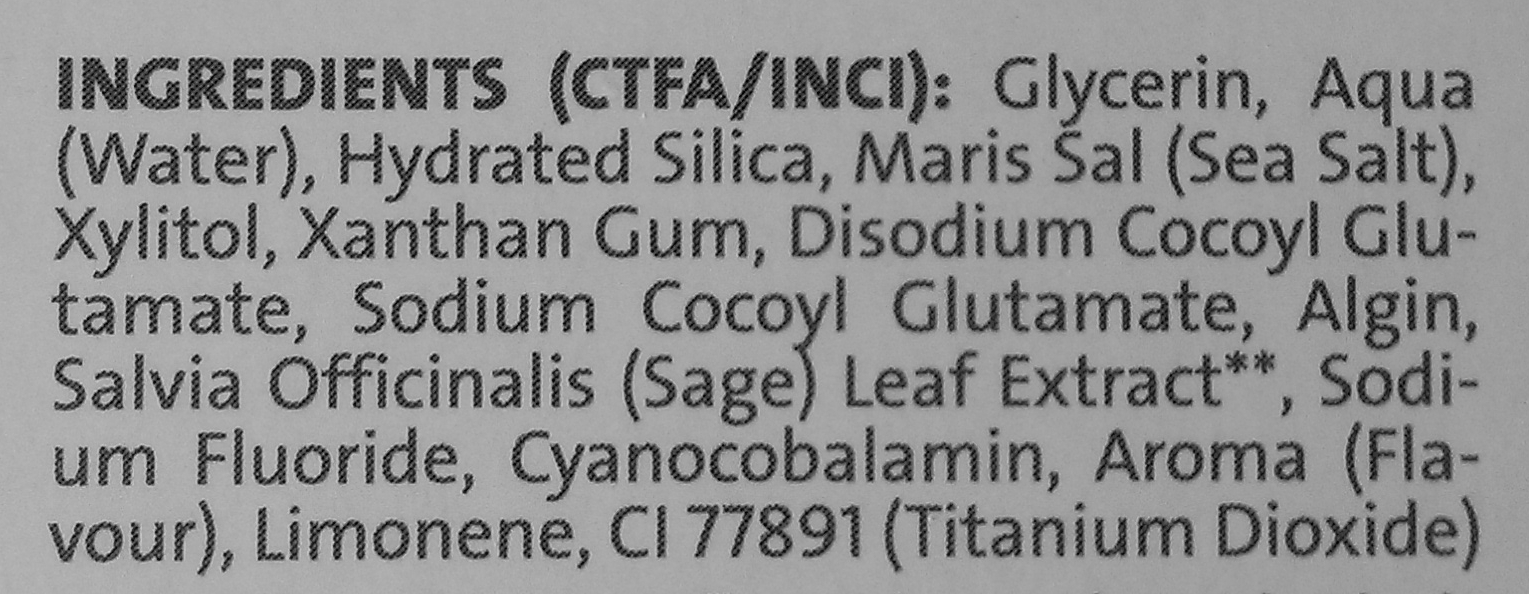
\includegraphics[scale=0.2]{pics/ingredient_list.jpg}
	\caption[Schwer verständliche Zutatenliste
	am Beispiel der Zahncreme "`Vitamin B12"' von "`Sante"']{Schwer verständliche Zutatenliste
	am Beispiel
	der Zahncreme "`Vitamin B12"' von "`Sante"', selbst fotografiert}
	\label{img:ingredient_list}
\end{figure}

Eine Kampagne der Verbraucher*innenorganisation\,\footnote{Die
Sprachform dieser Arbeit (mit Asterisk) versucht einseitige
Sprachformen zu transzendieren und inkludiert auch Menschen abseits
des binären Geschlechtermodells \citeweb{scilogs, asterisk}.}
"`Foodwatch"' hat diese
Probleme aufgezeigt, mit denen u.\,a. vegan oder vegetarisch lebende Menschen
konfrontiert werden. So werden z.\,B. Auszüge aus Schweineborsten/Federn zum Behandeln von
Mehl oder tierische Bestandteile als Trägerstoffe für Aromen oder
Vitamine benutzt \citeweb{foodwatch}.\\
Möglich macht dies u.\,a. das Gesetz, welches eine Volldeklaration aller
Zutaten nicht vorschreibt \citeweb{bnn}.
Zusätzlich zu dieser fehlenden Volldeklaration steht -- sofern kein
Siegel oder Label dazu aufgedruckt ist -- auch nicht auf der Packung, ob an
einem Produkt oder Inhaltsstoffen davon Tierversuche \citeweb{agt}
durchgeführt wurden bzw. werden oder ob z.\,B. das oben erwähnte Verfahren,
das Klären von Wein mit Hilfe von tierischem Eiweiß, bei der
Herstellung angewendet wurde.\\
Diese fehlenden Informationen machen einen Einkauf für
Verbraucher*innen, für die diese Dinge relevant sind, nicht gerade
einfach.\\
Abhilfe schaffen dabei Anfragen an die Hersteller*innen, ob ein Produkt
bspw. vegan ist oder nicht. Diese liegen aber bislang
verstreut auf Blogs oder Foren vor, wenn sie überhaupt
veröffentlicht wurden.\\
Zudem gibt es keine Produktdatenbank mit freien Daten, die einfach
verwendet bzw. erweitert werden könnte.

Die vorliegende Arbeit soll diese Lücke füllen, indem sie zu
einem Produkt entsprechende Informationen (mit Quellen bzw. Belegen)
bereitstellt, welche im Supermarkt z.\,B. via Smartphone
abgerufen werden können.
Es stellt sich dabei die Frage, wie eine Produktdatenbank aufgebaut
werden kann, die Produkt- und andere Informationen zentral sammelt und auf
Grundlage dieser Daten automatisch ermitteln kann, ob ein Produkt
vegan ist oder nicht und wie diese Daten für alle frei verfügbar
gemacht werden und plattformunabhängig einsehbar sein können.

\section{Ziel der Arbeit}
\label{sec:aim}

Das Ziel dieser Arbeit ist der Aufbau einer frei verfügbaren
Produktdatenbank,
um ähnliche oder darauf aufbauende Arbeiten zu vereinfachen und so
zu vermeiden, dass jedes Mal alle Informationen erneut zusammengesucht
und gespeichert werden müssen.
Diese Produktdatenbank soll
plattformunabhängig per Website und mobiler App erreichbar sein und von
der Community, d.\,h. den Nutzer*innen aufgebaut werden.
Der Fokus liegt dabei auf Veganismus, so soll automatisch bestimmt
werden, ob ein Produkt
vegan ist oder nicht.\\
Realisiert werden soll dies mit Hilfe einer Webanwendung und
den dazugehörigen mobilen Apps, wobei die Daten von den Nutzer*innen
verwaltet werden können und bei Eingabe eines Produktnamens oder der
zur Identifikation dienende Barcode
Produktinformationen und insbesondere
Informationen darüber, ob und wie das Produkt vegan ist oder
nicht
angezeigt werden.

\section{Aufbau der Arbeit}

In Kapitel \ref{chap:introduction} wurde die Motivation und das Ziel
dieser Arbeit beschrieben.\\
Kapitel \ref{chap:fundamentals} erklärt grundlegende Begriffe,
darunter woher der Veganismus stammt und wie
Veganismus und damit zusammenhängende Begriffe in dieser
Arbeit definiert werden. Zudem werden
technische Grundlagen erläutert, die im vorliegenden Werk verwendet
werden.\\
In Kapitel \ref{chap:related_work} wird die vorliegende Arbeit mit
ähnlichen Arbeiten bzw. Angeboten anhand verschiedener Kriterien
verglichen und die Ergebnisse zusammengefasst.\\
Kapitel \ref{chap:concept} stellt das Konzept dieser Arbeit
detailliert vor, darunter die Anforderungen, die gestellt werden und
wie diese gelöst werden können.\\
Kapitel \ref{chap:implementation} behandelt die Implementierung.
Es wird beschrieben, wie das in Kapitel \ref{chap:concept} vorgestellte
Konzept umgesetzt wurde und wie diese Arbeit in das
\ac{IRL}
integriert wurde \citeweb{irl}, \cite{sskk09}.\\
Kapitel \ref{chap:disc_eval} diskutiert die aus der Implementierung
resultierende Webanwendung und mobile App und evaluiert diese
anhand dem Feedback der Tester*innen.\\
In Kapitel \ref{chap:summ_futu} wird schließlich die Arbeit
zusammengefasst und es werden diverse Möglichkeiten vorgestellt, was
auf Grundlage dieser Arbeit noch alles entwickelt, bzw.
wie sie weiterentwickelt werden kann.



\chapter{Grundlagen}
\label{chap:fundamentals}

Im Folgenden wird der Begriff "`Veganismus"' und damit zusammenhängende
Begriffe beschrieben bzw. definiert. Ebenso werden technische
Hilfsmittel, die in dieser Arbeit Verwendung finden, erläutert.

\section{Veganismus}

Das Wort vegan leitet sich von dem englischen Wort vegetarian ab und
wurde erstmals 1944 von Donald Watson publiziert \cite[S. 2]{wat44}.
Es sollte eine klare Abgrenzung zu den `klassischen'
Ovo-Lakto-Vegetarier*innen sein \cite[S. 75\,f.]{bre05}.\\
Veganismus bezeichnet eine Lebensweise, bei der der Konsum aller
Tierprodukte abgelehnt wird. Darunter fallen u.\,a. nicht nur Fleisch, Fisch,
Eier, Milchprodukte, Honig und versteckte Tierprodukte wie z.\,B. mit
Gelatine geklärte Säfte, sondern auch Kleidung und
Gebrauchsgegenstände wie Leder, Pelz, Daunen, Seide, Perlen, Hörner,
usw.
Zudem werden Tierversuche vor allem im Kosmetikbereich aber auch
generell und
die Zurschaustellung von Tieren z.\,B. im Zirkus, Zoo und
Tierkampf abgelehnt \cite[S. 74]{bre05}.\\
Der \ac{VEBU} geht im Moment (Juli 2013) von rund 7 Millionen
Vegetarier*innen (8-9\,\% der Bevölkerung) und etwa 800.000
Veganer*innen in Deutschland aus \citeweb{vebu:anzahl}.

\subsection{Abgrenzung}

Da der Begriff Veganismus nicht klar abgegrenzt ist und von
jeder Person nach dem Motto "`Vermeide das Vermeidbare"' selbst
festgelegt werden kann, erfolgt hier eine Definition, was im Folgenden
als vegan angesehen werden soll.

Im Folgenden bedeutet vegan, dass:
\begin{itemize}
	\item keine tierischen Stoffe im Produkt vorhanden sind, auch
			keine undeklarierten
	\item keine tierischen Produkte im Herstellungsprozess verwendet
			wurden
\end{itemize}

Streng genommen sind auch folgende Verfahren unvegan:
\begin{itemize}
	\item Düngung mit tierischen Produkten, z.\,B.
			Hirschhornsalz
	\item Tierversuche, z.\,B. für Kosmetika
	\item Herstellung oder Gebrauch von unveganen Verpackungsmaterialien, z.\,B.
			kaseinhaltiger Kleber bei Etiketten
	\item Rodung von Urwäldern bzw. Feldern zur Gewinnung von Rohstoffen, z.\,B.
			Palmöl, da dabei Tiere und deren Lebensräume zerstört
			werden
	\item Herstellung von veganen Produkten mit Spuren von tierischen
			Produkten, die als Warnung vor Kreuzkontaminationen bei
			Allergiker*innen angegeben werden müssen
\end{itemize}

Da diese Verfahren aber nur schwer zu kontrollieren sind und ihre 
Einbeziehung daher zu weit
führen würde, wird sich auf die obige Definition
beschränkt\,\footnote{In den Produktanfragen oder den Kommentaren kann dazu aber natürlich
nachgefragt bzw. kommentiert werden bzw. es kann ein Produkt gekauft
werden, bei dem dies nicht der Fall ist.}
\citeweb{maqi:vegan}.

\subsection{Produktanfrage}
\label{sec:inquiry}

Um herauszufinden, ob ein Produkt wirklich vegan ist, wird
üblicherweise eine sogenannte Produktanfrage an die Hersteller*innen
gestellt. Dies ist normalerweise eine einfache E-Mail mit genauen Fragen z.\,B. nach
den Inhaltsstoffen oder der Herstellung.
Durch die Verbreitung der sozialen Netzwerke können Produktanfragen
auch direkt auf z.\,B. der "`Fanpage"' bei Facebook von einem Unternehmen gestellt
werden. Ein Vorteil dabei ist die höhere Aufmerksamkeit, die bei einer
E-Mail meist nicht gewährleistet ist.
Eine Alternative ist das Kontaktformular auf der Website des
Unternehmens, welches das Produkt herstellt, sofern keine
E-Mailadresse angegeben ist.\\
Eine beispielhafte Produktanfrage, wie sie auch in dieser Arbeit
verwendet bzw. automatisch generiert wird, befindet sich im Anhang (siehe
\ref{appendix:inquiry}).
Diese Produktanfrage wurde mit Hilfe des Baukastensystems auf der
Website der Tierrechtsinitiative Maqi erstellt
\citeweb{maqi:inquiry}.

\subsection{Veganität}
\label{sec:veganity}

Der Begriff Veganität wurde schon in der Einleitung (siehe
Abschnitt~\ref{sec:aim}) erwähnt, soll hier
aber noch genauer definiert werden.
Im Prinzip bedeutet Veganität, wie bzw. ob ein Produkt vegan ist.
Dabei kann Veganität in die vier Kategorien "`vegan"', "`unvegan"',
"`unklar"' und "`unbekannt"' eingeteilt
werden, die in Tabelle~\ref{table:veganity} näher erläutert sind und so auch
in dieser Arbeit benutzt werden.

\begin{table}[ht]%
\rowcolors{2}{gray!25}{white}
\centering
\begin{tabular}{c|m{12cm}}
\rowcolor{gray!50}
\textbf{Kategorie} & \textbf{Erläuterung}\\
\hline
vegan & \begin{itemize}[noitemsep]
	\item es befinden sich keine tierischen Zutaten in dem Produkt
	\item bei der Herstellung wurden keine tierischen Produkte verwendet
	\item die Angaben der Hersteller*in sind vollständig, d.\,h. es
			wurden alle Fragen ausreichend genau beantwortet
	\item es wurde seit der letzten Produktanfrage nichts an der
			Herstellung oder den Zutaten geändert
\end{itemize}\\
unvegan & \begin{itemize}[noitemsep]
	\item es befindet sich mindestens eine unvegane Zutat in dem
Produkt
	\item es wurde mindestens ein tierischer Stoff in der Herstellung
			verwendet
\end{itemize}\\
unklar & \begin{itemize}[noitemsep]
	\item mindestens eine Zutat ist unklar bzgl. der Veganität
	\item es wurden noch nicht alle Fragen geklärt
	\item die Angaben weichen von anderen Quellen ab oder sind
			veraltet
\end{itemize}\\
unbekannt & es liegen keine näheren Informationen zu dem Produkt vor,
insbesondere keine Zutatenliste
\end{tabular}
\caption[Einteilung der Veganität in vier Kategorien]{Einteilung der Veganität 
in vier
Kategorien \citeweb{maqi:categories}}
\label{table:veganity}
\end{table}%

Woraus sich die Veganität in dieser Arbeit genau zusammensetzt und wie
sie berechnet wird, wird im Konzept (siehe Kapitel \ref{chap:concept}) und der
Implementierung (siehe Kapitel \ref{chap:implementation}) beschrieben.

\section{Technische Grundlagen}

Um das bestehende System zur Identifikation von Produkten zu benutzen,
was u.\,a. in allen Einzelhandelsketten existiert, wird im Folgenden die
Funktionalität des Barcodes und eines Barcodescanners beschrieben.\\
Anschließend wird die Software PhoneGap genauer betrachtet, mit der
sich solch ein Scanner schnell und einfach für mehrere mobile Betriebssysteme bauen
lässt, um die Plattformunabhängigkeit zu gewährleisten.\\
Zum Schluss wird ein Authentifizierungsverfahren beschrieben, mit dem sich
Nutzer*innen auf der Website anmelden können, um die Produktdaten zu
verwalten.

\subsection{Barcode und -Scanner}
\label{sec:barcode}

Durch einen Barcode (auch Strichcode oder Balkencode genannt), der nur
eine Nummer in einem maschinenlesbaren Code enthält, können
Produkte identifiziert werden. Ein Beispiel-Barcode ist in Abbildung
\ref{img:4019339506035} zu sehen.

% barcode -E -b "4019339506035" -o 4019339506035.eps
\begin{figure}[ht]
	\centering
	
\includegraphics{pics/4019339506035.eps}
	\caption{Beispiel-Barcode: Kressesamen der Firma Davert}
	\label{img:4019339506035}
\end{figure}

Barcodes werden u.\,a. im Lebensmittelhandel benutzt, um Produkte
weltweit eindeutig zu kennzeichnen und z.\,B. Preisen und anderen
Informationen zuordnen zu können.
Diese werden u.\,a. in Form einer \ac{GTIN}, worin auch die früher
genutzte \ac{EAN} enthalten ist,
von der Organisation \ac{GS1}
vergeben und verwaltet \citeweb{gs1}.
Informationen zu einer \ac{GTIN} können z.\,B. über die 
offizielle Datenbank der \ac{GS1} (GEPIR) oder über eine freie
Datenbank, z.\,B. "`OpenGTINDB"', eingeholt werden \citeweb{gs1:gepir,
opengtindb}.\\
Ein Barcode wie z.\,B. \texttt{\textbf{4019339506035}} mit der
Codierung "`EAN-13"' setzt sich dabei wie folgt
zusammen:

\begin{itemize}
	\item \texttt{\textbf{401}}: Länderpräfix für Deutschland \citeweb{gs1:prefixlist}
	\item \texttt{\textbf{9339}}: Betriebsnummer des Herstellers, wird von
			\ac{GS1} vergeben, kann auch aus 5 oder
6 Stellen bestehen
	\item \texttt{\textbf{50603}}: Artikelnummer, wird vom Hersteller vergeben,
			abhängig von der Länge der Betriebsnummer 3 bis 5 Stellen
	\item \texttt{\textbf{5}}: Prüfziffer
\end{itemize}

Auch in dieser Arbeit wird der Barcode als Identifikationsmittel
verwendet.

\subsection{PhoneGap}
\label{sec:phonegap}

PhoneGap ist eine freie Software von Adobe, mit der eine native \ac{App}
für alle gängigen mobilen Betriebssysteme (u.\,a. iOS und Android)
erstellt werden kann, ohne jeweils eine eigene App in der jeweiligen
Sprache zu schreiben \citeweb{adobe:phonegap:about}.
Dazu wird einfach eine Webanwendung mit HTML5, CSS3 und JavaScript
(bzw. JavaScript-Bibliotheken)
erstellt und PhoneGap sorgt zusammen mit PhoneGap Plugins dafür, dass mit
JavaScript auf native Komponenten des mobilen Geräts (wie z.\,B. die
Kamera) zugegriffen werden kann.
Dieses Verfahren ist in der Übersicht
in Abbildung~\ref{img:phonegap} dargestellt.

\begin{figure}[ht]
	\centering
	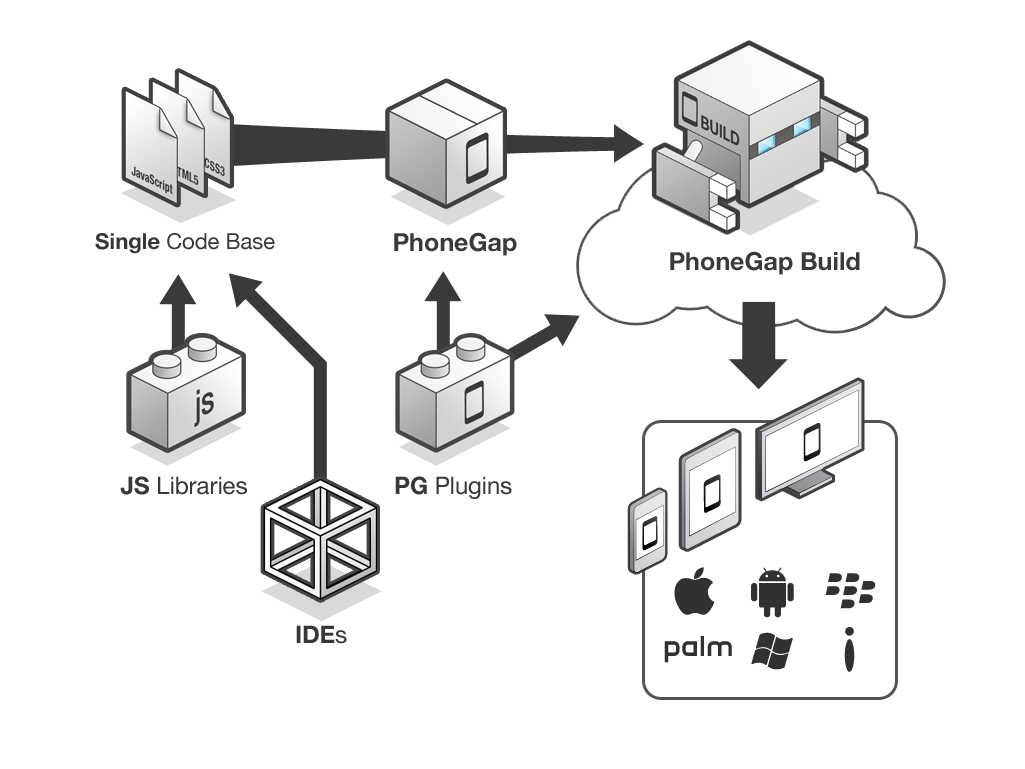
\includegraphics[scale=0.35]{pics/phonegap_build-diagram-2.png}
	\caption[Die Funktionalität von PhoneGap in der Übersicht]{Die Funktionalität von
			PhoneGap in der Übersicht \citeweb{adobe:phonegap:diagram}}
	\label{img:phonegap}
\end{figure}

Für diese Arbeit werden hauptsächlich die Komponenten Netzwerk und
Kamera benötigt, die bei allen Systemen unterstützt werden
\citeweb{adobe:phonegap:features}. Ein PhoneGap Plugin sorgt zusammen
mit diesen Komponenten dafür, dass
ein Barcode mit einer solchen \ac{App} gescannt werden kann.

\subsection{OAuth}
\label{sec:oauth}

OAuth ist ein Verfahren, durch welches das Registrieren bei vielen
verschiedenen Websites erleichtert wird, indem sich mit einer
"`offenen Identität"' angemeldet wird, die von einem Provider wie z.\,B.
Google,
bereitgestellt wird \citeweb{google:oauth}.
Dadurch entfallen für Entwickler*innen z.\,B. die Speicherungen von
Passwörtern, die teilweise immer noch mit alten Verfahren
verschlüsselt werden.
Nutzer*innen haben dadurch den Vorteil, sich nicht noch einen
Anmeldenamen und das dazugehörige Passwort zu merken.\\
In dieser Arbeit wird dieses Verfahren zum Anmelden benutzt, um
anschließend neue Produkte eintragen zu können oder schon vorhandene
zu ändern.
